\documentclass{article}
\usepackage[utf8]{inputenc}
\usepackage{tikz}
\usepackage{amssymb,amsmath, amsfonts, amsthm}
\usepackage{url}
\usepackage{cancel}
\usepackage[margin=1.5in]{geometry}
\usepackage{mathtools}
\usepackage{caption, subcaption}
\usepackage{pgf}
\usetikzlibrary{arrows, automata}
\usepackage{verbatim}
\usepackage{enumitem}
\usepackage{xcolor}

\newlength\tindent
\setlength{\tindent}{\parindent}
\setlength{\parindent}{0pt}
\renewcommand{\indent}{\hspace*{\tindent}}


{\theoremstyle{plain}
	\newtheorem{theorem}{Theorem}[section]
	\newtheorem*{theorem*}{Theorem}
	\newtheorem{conjecture}[theorem]{Conjecture}
	\newtheorem{proposition}[theorem]{Proposition}
	\newtheorem{lemma}[theorem]{Lemma}
	\newtheorem{corollary}[theorem]{Corollary}
}
{\theoremstyle{definition}
	\newtheorem{definition}[theorem]{Definition}
	\newtheorem*{definition*}{Definition}
	\newtheorem{remark}[theorem]{Remark}
	\newtheorem{example}[theorem]{Example}
	\newtheorem{question}[theorem]{Question}
	\newtheorem{hypotheses}[theorem]{Hypotheses}
	\newtheorem{hypothesis}[theorem]{Hypothesis}
}

\newcommand{\R}{{\mathbb{R}}}
\DeclareMathOperator*{\argmin}{arg\,min}
\DeclareMathOperator*{\argmax}{arg\,max}

\title{Independent Study 2018}
\author{Ziyan (Jessica) Feng, Nhu Do}
\date{\today}

\begin{document}
\maketitle

\section{Introduction}

\section{Mathematical background}
\subsection{The Lagrange dual function}

\subsubsection{The Lagrangian}

Consider an optimization in standard form:

\begin{equation} \label{eq:1}
\begin{array}{l}
\textrm{minimize:	 }  f_0(x) \\
\textrm{subject to:  } 
f_i(x) \le 0, \hspace*{1cm} i = 1, \ldots, m \\
\hspace{1.8cm} h_i(x) = 0, \hspace*{1cm} i = 1, \ldots, p, 
\end{array}
\end{equation}

with variable $x \in \mathbb{R}^n$. Assume its domain $\mathcal{D}$ is nonempty, and denote by $p^*$ the optimal value of problem (\ref{eq:1}), which is not necessarily convex.\\

The basic idea in Lagrangian duality is to augment the objective function with a weighted sum of the constraint functions. We defined the \textit{Lagrangian} $L: \R^n \times \R^m \times \R^p \rightarrow \R$ associated with this problem as:
$$ L(x,\lambda,\nu) = f_0(x) + \sum_{i=1}^m \lambda_i f_i(x) + \sum_{i=1}^p \nu_i h_i(x) $$
with domain $L = \mathcal{D} \times \R^m \times \R^p$. We refer to $\lambda_i$ as the \textit{Lagrange multiplier} associated with the $i$th inequality constraint, and $\nu_i$ the Lagrange multiplier associated with the $i$th equality constraint. Vectors $\lambda, \nu$ are the \textit{dual variables} or \textit{Lagrange multiplier vectors}. 

\subsubsection{The Lagrange dual function}

We define the \textit{Lagrange dual function} $g: \R^m \times \R^p \rightarrow \R$ as the minimum value of the Lagrangian over $x$: 
$$  g(\lambda,\nu) = \inf_{x \in \mathcal{D}} L(x, \lambda, \nu) = \inf_{x \in \mathcal{D}} \left(f_0(x) + \sum_{i=1}^m \lambda_i f_i(x) + \sum_{i=1}^p \nu_i h_i(x) \right)$$

As $g$ is the pointwise infimum of a family of affine functions of $(\lambda,\nu)$, it is concave.
	
\subsubsection{Lower bounds on optimal value}
Let's denote by $x \succeq y$ the componentwise inequality between vectors x and y. 

The dual function yields lower bounds on the optimal value $p^*$ of problem (\ref{eq:1}): For any $\lambda \succeq 0$ and any $\nu$ we have: 
\begin{equation} \label{eq:2}
g(\lambda,\nu) \le p^*,
\end{equation}
which can be easily verified. The dual function gives a nontrivial lower bound on $p^*$ only when $\lambda \succeq 0$ and $g(\lambda,\nu) > -\infty.$ Such a pair $(\lambda,\nu)$ is called \textit{dual feasible}.

\subsubsection{Linear approximation interpretation}

We can rewrite the original problem (\ref{eq:1}) as an unconstraine problem,
\begin{equation} \label{eq:unconstrained}
\textrm{minimize } f_0(x) + \sum_{i=1}^m I_f(f_i(x)) + \sum_{i=1}^p I_0 (h_i(x)), 
\end{equation}
where:
$$I_f(u) = 
\begin{cases}
0, \hspace{0.4cm} u \le 0\\
+\infty, \hspace{0.1cm} u > 0
\end{cases}, \hspace{0.2cm}
I_g(u) = 
\begin{cases}
0, \hspace{0.4cm} u = 0\\
+\infty, \hspace{0.2cm} u \neq 0
\end{cases}$$

The function $I_f(u), I_g(u)$ can be interpreted as expressing our displeasure associated with the violation of the corresponding constraint.

We can approximate problem (\ref{eq:unconstrained}) as minimizing the Lagrangian $L(x, \lambda, \nu)$, and the dual function value $g(\lambda, \nu)$ is the optimal value of the problem
\begin{equation} \label{eq:Lagrangian}
\textrm{minimize } L(x,\lambda,\nu)  = f_0(x) + \sum_{i=1}^m \lambda_i f_i(x) + \sum_{i=1}^p \nu_i h_i(x) 
\textrm{, assuming all } \lambda_i > 0
\end{equation}

Since $\lambda_i u \le I_f(u)$ and $\nu_i u \le I_0(u)$ for all $u$, it's clear that the dual function yields a lower bound on the optimal value of the original problem. 

% \subsubsection{The Lagrange dual function and conjugate functions}

% The conjugate $f^*$ of a function $f: \R^n \rightarrow \R$ is given by
% $$f^*(y) = \sup_{x \in \text{ dom } f} (y^T x - f(x))$$

% Consider an optimization problem with linear inequality and equality constraints: 
% \begin{equation} \label{cjg}
% \begin{array}{l}
% \textrm{minimize:	 }  f_0(x) \\
% \textrm{subject to:  } 
% Ax \preceq b \\
% \hspace{1.8cm} Cx = d
% \end{array}
% \end{equation}

% Using the conjugate of $f_0$, the dual function for problem (\ref{cjg}) is:
% $$g(\lambda,\nu) = -b^T \lambda - d^T \nu - f_0^*(-A^T \lambda - C^T \nu)$$

% The domain of $g$ follows from the domain of $f_0^*$:

% $$\text{dom } g = \{(\lambda,\nu) | -A^T \lambda - C^T \nu \in \text{ dom } f_0^* \}$$

\subsubsection{The Lagrange dual problem}

For each pair $(\lambda, \nu)$ with $\lambda \succeq 0$, the Lagrange dual function gives us a lower bound on the optimal value $p^*$ of the optimization problem (\ref{eq:1}). The best lower bound can be found by solving the optimization problem:
\begin{equation} \label{eq:dual}
\begin{array}{l}
\textrm{maximize: } g(\lambda, \nu)\\
\textrm{subject to: } \lambda \succeq 0.
\end{array}
\end{equation}

This problem is called the \textit{Lagrange dual problem} associated with problem (\ref{eq:1}). The original problem (\ref{eq:1}) is called the \textit{primal problem}. We refer to $(\lambda^*, \nu^*)$ as \textit{dual optimal} or \textit{optimal Lagrange multipliers}.

The Lagrange dual problem (\ref{eq:dual}) is a convex optimization problem, since the objective function is concave and the constraint is convex. This is the case regardless of whether the primal problem is convex.

\subsubsection{Weak duality and Strong duality}
The optimal value of the Lagrange dual problem, which we denote $d^*$, is, by definition, the best lower bound on $p^*$ that can be obtained from the Lagrange dual function. In particular, we have:
\begin{equation}\label{eq:weak}
d^* \le p^* ,
\end{equation}
This property is called \textit{weak duality}. The inequality (\ref{eq:weak}) holds when $d^*$ and $p^*$ are infinite. The bound (\ref{eq:weak}) is sometimes used to find a lower bound on the optimal value of a problem that is difficult to solve, since the dual problem is always convex, and in many cases can be solved efficiently. \newline

If the equality
\begin{equation} \label{eq:strong}
d^* = p^*
\end{equation}
holds, then we say that \textit{strong duality} holds. \\

In general, strong duality does not hold. But if the primal (\ref{
eq:1}) is convex, we usually (though not always) have strong duality. \\

A condition that guarantee strong duality is \textit{Slater's condition}: there exists an $x \in $ \textbf{relint} $\mathcal{D}$ such that 
\begin{equation}\label{eq:Slater}
f_i(x) < 0, i = 1, \ldots, m, \hspace{0.5cm} Ax = b.
\end{equation}
where  \textbf{relint} $\mathcal{D}$ denotes the relative interior of $\mathcal{D}$. Slater's theorem states that strong duality holds, if Slater's condition holds, and the problem is convex. Besides, the affine inequalities do not need to hold with strict inequality. Slater's condtion also implies that dual optimal value is attained when $d^* > - \infty$, i.e., there exists a dual feasible $(\lambda^*, \nu^*)$ with $g(\lambda^*,\nu^*) = d^* = p^*$.

\subsection{Optimality conditions}

\subsubsection{Complementary slackness}
Suppose that the primal and dual values are attained and equal (so strong duality holds). Let $x^*$ be a primal optimal and $(\lambda^*, \nu^*)$ be a dual optimal point. There are some important observations: 
\begin{itemize}
	\item $x^*$ minimizes $L(x,\lambda^*,\nu^*)$ over $x$ (The Lagrangian $L(x,\lambda^*, \nu^*)$ can have other minimizers, $x^*$ is simple a minimizer).
	\item \textit{Complementary slackness:} $\lambda_i^* f_i(x^*) = 0$, for $ i = 1, \ldots, m.$
\end{itemize}

\subsubsection {KKT optimality conditions}
Assume that the functions $f_0, f_1, \ldots, f_m, h_1, \ldots, h_p$ are differentiable. \newline

\textbf{KKT conditions for nonconvex problem}

Since $x^*$ minimizes $L(x,\lambda^*, \nu^*)$ over $x$, by first-order necessary condition for a minimum, its gradient must vanish at $x^*$, i.e.,
$$\nabla f_0(x^*) + \sum_{i=1}^m \lambda_i^* \nabla f_i(x^*) + \sum_{i=1}^p \nu_i^* \nabla h_i(x^*) = 0$$.

Thus we have
\begin{align*}
f_i(x^*) & \le 0, i = 1, \ldots, m\\
h_i(x^*) & = 0, i = 1, \ldots, p\\
\lambda_i^* & \ge 0, i = 1, \ldots, m\\
\lambda_i^* f_i(x^*) & = 0, i = 1, \ldots, m \\
\nabla f_0(x^*) + \sum_{i=1}^m \lambda_i^* \nabla f_i(x^*) + \sum_{i=1}^p \nu_i^* \nabla h_i(x^*) &= 0
\end{align*}
which are called the \textit{Karush-Kuhn-Tucker} (KKT) conditions. \newline

For any optimization problem with \textbf{differentiable} objective and constraint functions for which \textbf{strong duality} obtains, any pair of primal and dual optimal points must satisfy the KKT conditions.\newline

\textbf{KKT conditions for convex problems}

When the primal problem is convex, if $f_i$ are convex and $h_i$ are affine, and $\widetilde{x}, \widetilde{\lambda}, \widetilde{\nu}$ are points that satisfy the KKT conditions, then $\widetilde{x}$ and $(\widetilde{\lambda},\widetilde{\nu})$ are primal and dual optimal. 

If a convex optimization problem with differentiable objective and constraint functions satisfies Slater's condition, then the KKT conditions proves necessary and sufficient conditions for optimality.

\subsection{Augmented Lagrangian and the Method of Multipliers}
Consider the problem: \begin{equation} \label{eq:MM}
\begin{array}{l}
\textrm{minimize:	 }  f(x) \\
\textrm{subject to:  } 
Ax = b
\end{array}
\end{equation}

The augmented Lagrangian for this problem is: 
$$L_{\rho}(x,\nu) = f(x) + \nu^T(Ax - b) + (\rho/2) \cdot||Ax - b||^2$$
where $\rho > 0$ is called the \textit{penalty parameter}. Note that $L_0$ is the standard Lagrangian for the problem.

The algorithm: 

\begin{equation}\label{eq:MMx}
    x^{k+1} = \text{argmin}_{x} L_\rho(x,\nu^k) 
\end{equation}
\begin{equation}
    \nu^{k+1} = \nu^k + \rho(Ax^{k+1} - b)
\end{equation}

is the  \textit{Method of Multipliers} for solving (\ref{eq:MM}). This is the same as standard dual ascent, but the $x-$minimization step uses the augmented Lagrangian, and the penalty parameter $\rho$ is used as the step size. The method of multipliers converges under far more general conditions than dual ascent. By using the $\rho$ as the step size in the dual update, the iterate $(x^{k+1}, \nu^{k+1})$ is dual feasible. As the method of multipliers proceed, the primal residual $Ax^{k+1} - b$ converges to zero, yielding optimally. \newline

Disadvantage: When $f$ is separable, the augmented Lagrangian $L_{\rho}$ is not separable, so the $x-$minimization step (\ref{eq:MMx}) cannot be carried out separately in parallel for each $x_i$.\\
(We say that $f$ is \textit{separable} (with respect to a partition or splitting of the variable into subvectors), meaning that $f(x) = \sum_{i=1}^N f_i(x_i)$ where $x = (x_1, \ldots, x_N)$ and the variables $x_i \in \R^{n_i}$ are subvectors of $x$).

\subsection{Alternating Direction Method of Multipliers (ADMM)}
\subsubsection{Algorithm}
ADMM solves problems in the form 

\begin{equation} \label{eq:3.1}
\begin{array}{l}
\textrm{minimize:	 } f(x)+g(z) \\
\textrm{subject to:  } Ax + Bz = c
\end{array}
\end{equation}
with variables $x \in \R^n, z \in \R^m$, where $A \in \R^{p \times n}, B \in \R^{p \times m}$, and $c \in \R^p$. The optimal value of this problem will be denoted by
$$p^* = \inf \{f(x)+g(z) \mid Ax + Bz = c \}$$
We form the augmented Lagrangian
$$L_{\rho}(x,z,y) = f(x)+g(z) + y^T(Ax+Bz-c) + \dfrac{\rho}{2}||Ax+Bz-c||^2$$

ADMM consists of the iterations
\begin{equation} 
\begin{array}{l}
x^{k+1} := \argmin\limits_x L_{\rho}(x,z^k,y^k)\\
z^{k+1} := \argmin\limits_z L_{\rho}(x^{k+1},z,y^k)\\
y^{k+1} := y^k + \rho(Ax^{k+1} + Bz^{k+1}-c)
\end{array}
\end{equation}
where $\rho > 0$.

\subsubsection{Convergence}
\textbf{Assumption 1.} The (extended-real-valued) functions $f:\R^n \rightarrow \R \cup \{+\infty\}$ and $g: \R^m \rightarrow \R \cup \{+\infty\}$ are closed, proper, and convex.\\
In other words, the function $f$ satisfies assumption 1 iff its epigraph 
$$\text{epi } f = \{(x,t) \in \R^n \times \R \mid f(x) \le t\}$$ is a closed nonempty convex set. Also note that $f,g$ could be nondifferentiable and assume the value $+\infty$.\\

\textbf{Assumption 2.} The unaugmented Lagrangian $L_0$ has a saddle point. Explicitly, there exist $(x^*, z^*, y^*)$, not necessarily unique, such that
$$L_0(x^*, z^*, y) \le L_0(x^*, z^*, y^*) \le L_0(x,z,y^*)$$ holds for all $x,z,y$.\\
This implies that $(x^*, z^*)$ is a solution to (\ref{eq:3.1}), $y^*$ is dual optimal, and the optimal values of the primal and dual problems are equal. \\

Under assumptions 1 and 2, the ADMM iterates satisfy the following:
\begin{itemize}
    \item \textit{Residual convergence.} $r^k \rightarrow 0$ as $k \rightarrow \infty$, where $r^k = Ax^k + Bz^k - c$, i.e., the iterates approach feasibility. \item \textit{Objective convergence.} $f(x^k) + g(z^k) \rightarrow p^*$ as $k \rightarrow \infty$, i.e., the objective function of the iterates approaches the optimal value. 
    \item \textit{Dual variable convergence.} $y^k \rightarrow y^*$ as $k \rightarrow \infty$, where $y^*$ is a dual optimal point.
\end{itemize}
Note that $x^k$ and $z^k$ need not converge to optimal values.

\section{Problem formulation}
Variables:
\begin{itemize}
    \item $b_i$: habitat target for species $i$
    \item $x_j$: amount of money invested for watershed $j$
    \item $f_j(x_j)$: total habitat in watershed $j$ if $x_j$ money is invested
    \item $a_{ij}$: whether species $i$ is available in watershed $j$\\
    $a_{ij} = 
    \begin{cases}
    1, \text{ if species i is in watershed j}\\
    0, \text{ otherwise}
    \end{cases}$
\end{itemize}
\textbf{Optimization problem}
\begin{align*}
    \min\ &\sum\limits_j x_j\\
    \text{subject to} \ & x_j \ge 0, \forall j \\
    &\sum\limits_j a_{ij}f_j(x_j)\ge b_i, \forall i
\end{align*}

\begin{itemize}
    \item Lagrangian: 
    \begin{equation}
        L(x,\lambda) = \sum\limits_j x_j + \sum\limits_i \lambda_i(b_i - \sum\limits_j a_{ij}f_j(x_j))
    \end{equation}
    \item Dual function:
    \begin{equation}
        g(\lambda) = \min\limits_{x \ge 0} L(x, \lambda)
    \end{equation}
    \item Dual problem:
    \begin{equation}\label{eq:dualprob}
        \max\limits_{\lambda \ge 0} g(\lambda)
    \end{equation}
\end{itemize}
\subsection{Gradient Ascent Approach}
The dual problem (\ref{eq:dualprob}) can be solved by using gradient ascent. \textbf{Gradient ascent} maximizes a function by moving in the positive gradient direction, or minimizes a function by moving in the negative gradient direction. 
$$ \max\limits_{\lambda \ge 0} g(\lambda)$$
$$\text{Gradient Ascent}: \lambda_{t+1} = \lambda_{t}+\alpha_{t}\nabla g(\lambda)$$
$$\nabla g(\lambda)=\nabla_{\lambda}L(x_{\lambda}^*, \lambda)=\sum\limits_{i} b_{i}-\sum\limits_{j} a_{ij} f_{j}(x_j)$$
where $x_\lambda^*$ is the minimizer of $L(x,\lambda)$.\newline
Gradient ascent produces $\lambda, \lambda^2\ldots \lambda^*$ that converges to $\lambda^*$. This is optimal for dual but not necessarily optimal for primal problem, since we get $x, x^2 \ldots x^*$ from $\lambda$.\newline\newline
\textbf{Project gradient ascent} minimize subject to a constraint by moving in the direction of negative gradient, then projecting onto feasible set. 
$$\max\limits_{\lambda \ge 0}g(\lambda)$$
$$y_{t+1} = \lambda_t+\alpha_t\nabla g(\lambda)$$
$$\lambda_{t+1}= \argmax\limits_{\lambda \ge 0}||y_{t+1}+\lambda_t||$$
Dual Ascent produces (both gradient ascent and project gradient ascent):
$$\lim_{t\to\infty}g(\lambda^{t})=g(\lambda^*)$$
We also want: 
$$\lim_{t\to\infty}f(x^{t})=f(x^*)$$
We can get $x_{\lambda}^*$ by using each $\lambda_t$, but can not prove primal is optimal. \newline
Thus gradient ascent can not solve our problem since we can only get optima for dual problem, and we can not prove strong duality. We will introduce another method, ADMM, in next section, which gives both $\lambda^*$ and $x^*$. 


\subsection{ADMM approach}
Assume that there are $m$ species and $n$ watersheds. We introduce slack variables $s_i$'s and rewrite the primal as follows:
\begin{align*}
\text{minimize } & \sum\limits_{j=1}^n x_j\\
\text{subject to } & \sum\limits_{j=1}^n  a_{ij} f_j(x_j) = b_i + s_i, \forall i=1, \ldots, m \\
& x_j \ge 0, \forall j=1,\ldots,n \\
& s_i \ge 0, \forall i=1,\ldots,m
\end{align*}

Let $A \in \R^{m \times n}$ such that $(A)_{ij} = a_{ij}$, $f(x) = 
\begin{bmatrix}
f_1(x_1) \\
\vdots \\
f_n(x_n)
\end{bmatrix}$, 
$b =
\begin{bmatrix}
b_1 \\
\vdots \\
b_m
\end{bmatrix}$,
$s = \begin{bmatrix}
s_1 \\
\vdots \\
s_m
\end{bmatrix}$. \newline



\begin{itemize}
\item The primal now becomes:
\begin{align*}
\text{minimize } & \sum\limits_{j=1}^n x_j\\
\text{subject to } & Af(x) = b + s \\
& x_j \ge 0, \forall j=1,\ldots,n \\
& s_i \ge 0, \forall i=1,\ldots,m
\end{align*}

\item Augmented Lagrangian: 
\begin{align*}
L_{\rho}(x,s,y) &= \sum\limits_{j=1}^n x_j + \sum\limits_{i=1}^m y_i(b_i+s_i- \sum\limits_{j=1}^n a_{ij}f_j(x_j)) + \dfrac{\rho}{2} \sum\limits_{i=1}^m \left(b_i + s_i-\sum\limits_{j=1}^n a_{ij}f_j(x_j)\right)^2\\
&= \sum\limits_{j=1}^n x_j + y^T(b + s - Af(x)) + \dfrac{\rho}{2}||b+s - Af(x)||^2
\end{align*}
note: $x$ and $s$ are primal variables, $y$ is dual variable. $y$ is unconstraint. 

\item Updating rule:\\
We first introduce some notations. In the $(k+1)$-th iteration that is updating vector $s$, let's say it is going to update component $s_i$ next. We denote by $s_{<i}^{k+1}$ values of the first $i-1$ components of vector $s$ that have been updated in the $(k+1)$-th iteration. Similarly, denote by $s_{>i}^k$ the last $m-i$ components of vector $s$ that have been updated in the $k$-th iteration, but not yet updated in the $(k+1)$-th iteration. Then we can write $s = 
\begin{bmatrix}
s^{k+1}_{<i} \\
--\\
s_i\\
--\\
s^{k}_{>i}
\end{bmatrix}$. We use similar notations for $x$ with $x_{<h},x_h$ and $x_{>h}$. 
The update rules are as follows:
\begin{itemize}
    \item[+] \underline{Update $x$}: (indexing match with for\_species function in Python code)   
    \begin{align*}
        x_j^{(k+1)} &= \argmin\limits_{x_j} L_{\rho}(x_{<j},x_j,x_{>j}, s^k, y^k)\\
        &= \argmin\limits_{x_j} \left\{ x_j - \sum\limits_{i=1}^m y_i^k \cdot a_{ij} \cdot f_j(x_j) + \dfrac{\rho}{2} \sum\limits_{i=1}^m  \left(b_i+s_i^k - \sum\limits_{h\neq j} a_{ih}f_h(x_h) - a_{ij}f_j(x_j) \right)^2 \right\}\\
        &= \argmin\limits_{x_j} \biggl\{x_j - f_j(x_j)\sum_{i=1}^m y_i^k a_{ij} + \\ 
        & \hspace{2cm} \dfrac{\rho}{2}\sum\limits_{i=1}^m \left[(a_{ij}f_j(x_j))^2 - 2a_{ij}f_j(x_j) \left(b_i+s_i^k-\sum\limits_{h < j}a_{ih}f_h(x_h^{k+1}) - \sum\limits_{h > j}a_{ih}f_h(x_h^k) \right) \right]  \biggr\} \\
        &= \argmin\limits_{x_j} \biggl\{x_j - f_j(x_j)\sum\limits_{i=1}^m y_i^k\cdot a_{ij}+\\
        & \hspace{2cm} \dfrac{\rho}{2}f_j(x_j)^2\sum\limits_{i=1}^m a_{ij}^2 - \rho\cdot f_j(x_j)\sum\limits_{i=1}^m a_{ij}\left(b_i+s_i^k - \sum\limits_{h<j}a_{ih}f_h(x_h^{k+1}) - \sum\limits_{h>j}a_{ih}f_h(x_h^k) \right) \biggr\}\\
        &= \argmin\limits_{x_j} \{x_j - \alpha\cdot f_j(x_j) + \beta \cdot f_j^2(x_j) \} \text{, where } \alpha \text { is unconstrained, } \beta > 0 \\
        &= \argmin\limits_{x_j} (F_{x_j})
    \end{align*}
    
    \item[+] \underline{Update $s$}:
    \begin{align*}
    s_i^{(k+1)} &= \argmin\limits_{s_i} L_{\rho}(x^{k+1},s_{<i},s_i,s_{>i},y^k) \\
    &= \argmin\limits_{s_i} \left[y_i^k s_i + \dfrac{\rho}{2}(b_i + s_i - (Af(x^{k+1}))_i)^2\right]\\
    &= \argmin\limits_{s_i} \left[y_i^k s_i + \dfrac{\rho}{2}(s_i^2 + 2b_is_i - 2s_i(Af(x^{k+1}))_i)\right]\\
    &= \argmin\limits_{s_i}\left[y_i^k s_i + \dfrac{\rho}{2}\left(s_i^2+2b_is_i - 2s_i\sum\limits_{j=1}^n a_{ij}f_j(x_j^{k+1})\right) \right]\\
    &= \argmin_{s_i} (F_{s_i})
    \end{align*}
    \item[+] \underline{Update $y$}: 
    \begin{align*}
        y^{k+1} = y^k + \rho \sum\limits_{i=1}^m \left(b_i+s_i^{k+1}-\sum\limits_{j=1}^na_{ij}f_j(x_j^{k+1})\right)
    \end{align*}
\end{itemize}
\item Square of convex function is also convex under certain condition\\
Let $g(x)$ be a convex function and $g(x)\ge 0\ \forall x$.\\
$\dfrac{d^2}{dx^2} \ge 0$ because $g(x)$ is convex.\\
Then \begin{align*}
    &\dfrac{d^2}{dx^2}(g(x))^2\\
    &=\dfrac{d}{dx} \left( 2g(x) \dfrac{d}{dx} g(x) \right)\\
    &=2\dfrac{d}{dx}g(x)\dfrac{d}{dx}g(x)+2g(x)\dfrac{d^2}{dx^2}g(x)\\
    &=2\left( \dfrac{d}{dx}g(x)\right)^2+2g(x)\dfrac{d^2}{dx^2}g(x)
\end{align*}
The square part is non-negative, $g(x)\ge 0$, and $\dfrac{d^2}{dx^2}g(x) \ge 0$. \\
Thus $\dfrac{d^2}{dx^2}(g(x))^2$. The square of a convex function is also convex. 


\item Convexity of the functions used to update components of $x, s$: 
\begin{itemize}
    \item[+] Because $f_h(x_h)$ is concave, bijective, and presumably strictly increasing, its inverse $f_h^{-1}(x_h)$ is convex. Besides, the function $-\alpha\cdot f_h(x_h) + \beta\cdot f_h^2(x_h)$ (view this as a function of $f_h(x_h)$) is convex (since $\beta>0$). Thus, $F_{x_h} = f_h^{-1}(x_h) + (-\alpha\cdot f_h(x_h) + \beta\cdot f_h^2(x_h))$ is convex.
    \item[+] $F_{s_i}$ is a quadratic function of $s_i$. Since $\dfrac{\rho}{2} > 0$, the function $F_{s_i}$ is convex. 
\end{itemize}
\item Checking KKT conditions for the formulation with slack variables:\\
(1) (We don't have inequality constraints) \\
(2) Checking $Af(x^*) \stackrel{?}{=} b + s^*$\\
(3) (We don't have dual variables that correspond to the inequality constraints)\\
(4) (No need to check complementary slackness since we don't have inequality constraints)\\
(5) Checking $\nabla f_0(x^*) + \sum\limits_{i=1}^m \lambda_i^* \nabla f_i(x^*) + \sum\limits_{i=1}^p \nu_i^* \nabla h_i(x^*) \stackrel{?}{=} 0$\\
For our formulation, and this condition becomes: \\
\begin{align*}
& \nabla (x_1 + \ldots + x_n + 0\cdot s_1 + \ldots + 0 \cdot s_m) - \sum\limits_{i=1}^m y_i^* \cdot \nabla \left(\sum\limits_{h=1}^n b_i+s_i-a_{ih} f_h(x_h) \right)  \\
= & \begin{bmatrix}
1 \\
\vdots\\
1\\
0\\
\vdots\\
0
\end{bmatrix}
-  \left( y_1^* \cdot 
\begin{bmatrix}
a_{11}\cdot f'_1(x_1) \\
\vdots\\
a_{1n} \cdot f'_n(x_n)\\
1\\
\vdots\\
0
\end{bmatrix} +
\ldots + 
y_m^* \cdot 
\begin{bmatrix}
a_{m1}\cdot f'_1(x_1) \\
\vdots\\
a_{mn} \cdot f'_n(x_n)\\
0\\
\vdots\\
1
\end{bmatrix} \right)\\
= &
\begin{bmatrix}
1 \\
\vdots\\
1\\
0\\
\vdots\\
0
\end{bmatrix} 
- 
\begin{bmatrix}
f'_1(x_1)\sum\limits_{i=1}^m y_i^*\cdot a_{i1} \\
\vdots\\
f'_n(x_n)\sum\limits_{i=1}^m y_i^*\cdot a_{in}\\
y_1^*\\
\vdots\\
y_m^*
\end{bmatrix} 
\hspace{0.6cm}
\stackrel{?}{\neq} 
\hspace{0.6cm}
\begin{bmatrix}
0 \\
\vdots\\
0\\
0\\
\vdots\\
0
\end{bmatrix} 
\end{align*}

\end{itemize}

\subsection{Deriving KKT conditions for our problem}

First, let's write a version of the problem that include Lagrange multipliers, i.e. dual variables, for the non-negativity constraints on $x$ and $s$. \newline

\begin{itemize}
\item\textbf{Primal}
\begin{align*}
\text{minimize } & \sum\limits_{j=1}^n x_j\\
\text{subject to } & \sum\limits_{j=1}^n  a_{ij} f_j(x_j) = b_i + s_i, \forall i=1, \ldots, m  \hspace*{1cm}(\text{duals: } y_1, \ldots, y_m: \text{ free})\\
& x_j \ge 0, \forall j=1,\ldots,n \hspace*{3.6cm} \color{red}(\text{duals: } w_1,\ldots,w_n \le 0) \\
& s_i \ge 0, \forall i=1,\ldots,m \hspace*{3.6cm} \color{red}(\text{duals: } z_1,\ldots,z_m \le 0)
\end{align*}
\item \textbf{Lagrangian}\\
$L(x,s,y,w,z) = \sum\limits_{j=1}^n x_j + \sum\limits_{i=1}^m y_i\left(b_i+s_i-\sum\limits_{j=1}^na_{ij}f_j(x_j)\right) \color{red} + \sum\limits_{j=1}^n w_j x_j + \sum\limits_{i=1}^m z_i s_i$
\item \textbf{KKT conditions for this version of the problem}\\
(1)
\begin{align*} &x_j\stackrel{?}{\ge} 0,\forall j=1,\ldots,n \\
& s_i\stackrel{?}{\ge} 0,\forall i=1,\ldots,m
\end{align*}
(2) Checking $Af(x^*) \stackrel{?}{=} b + s$\\
(3) Checking:
\begin{align*}
&w_j \stackrel{?}{\le} 0, \forall j=1,\ldots,n\\
&z_i \stackrel{?}{\le} 0, \forall i=1,\ldots,m
\end{align*}\\
(4) (Complementary slackness) 
\begin{align*}
&w_j x_j \stackrel{?}{=} 0,\forall j=1,\ldots,n\\ 
&z_is_i \stackrel{?}{=} 0,\forall i=1,\ldots,m
\end{align*} 
(5) (Stationary) (Is it correct that there are no stationary conditions for duals corresponding to inequality constraint, based on B\&V 5.5.3?)
\begin{align*}
    &\color{darkgray}\left(\dfrac{\partial L}{\partial x} \stackrel{?}{=} 0\right) \hspace*{1cm}
    \color{black}\begin{bmatrix}
1 \\
\vdots\\
1\\
\end{bmatrix} 
- 
\begin{bmatrix}
f'_1(x_1)\sum\limits_{i=1}^m y_i^*\cdot a_{i1} \\
\vdots\\
f'_n(x_n)\sum\limits_{i=1}^m y_i^*\cdot a_{in}\\
\end{bmatrix} 
+
\color{red}
\begin{bmatrix}
w_1\\
\vdots\\
w_n\\
\end{bmatrix}
\color{black}
\hspace{0.6cm}
\stackrel{?}{=} 
\hspace{0.6cm}
\begin{bmatrix}
0 \\
\vdots\\
0\\
\end{bmatrix}\\
 &\color{darkgray}\left(\dfrac{\partial L}{\partial s} \stackrel{?}{=} 0\right) \hspace*{1cm} \color{black} 
 \begin{bmatrix}
 y_1  \\
 \vdots\\
 y_m
 \end{bmatrix} + 
 \color{red} 
 \begin{bmatrix}
 z_1  \\
 \vdots\\
 z_m
 \end{bmatrix}
 \color{black}
 \hspace{0.6cm}
\stackrel{?}{=} 
\hspace{0.6cm}
\begin{bmatrix}
0 \\
\vdots\\
0
\end{bmatrix}
\end{align*}

\underline{Note}: $y$ is free, $w \le 0, z\le 0$

\subsubsection{KKT conditions for our problem}

(1)
\begin{align*} &x_j\stackrel{?}{\ge} 0,\forall j=1,\ldots,n \\
& s_i\stackrel{?}{\ge} 0,\forall i=1,\ldots,m
\end{align*}
(2) Checking $Af(x^*) \stackrel{?}{=} b + s$\\
(3) (Combining complementary slackness and Stationary conditions): 
\begin{itemize}
    \item If $x_j > 0$ for some $j$, we need to have: $1 = f'_j(x_j) \sum\limits_{i=1}^m y_i^* \cdot a_{ij}$.\\
    If $x_j = 0$ for some $j$, we only need: $1 \ge f'_j(x_j) \sum\limits_{i=1}^m y_i^* \cdot a_{ij}$.
    \item If $s_i > 0$ for some $i$, we need $y_i = 0$.\\
    If $s_i = 0$ for some $i$, $y_i$ can be anything.
    
\end{itemize}



\end{itemize}

\subsection{Experiments and Notes}

\subsubsection{Adjusting $\rho$}
In the original paper, there seems to be not enough information on how to set the penalty parameter $\rho$, which is used as the step size. We did several experiments on setting $\rho$ and recorded the number of iterations it takes to converge as well as performance on getting optimal solution. \\
We used the simple 3 species and 3 watersheds problem with the following a-matrix and b-vector $[1.5e+06, 3.5e+06, 3e+06]$

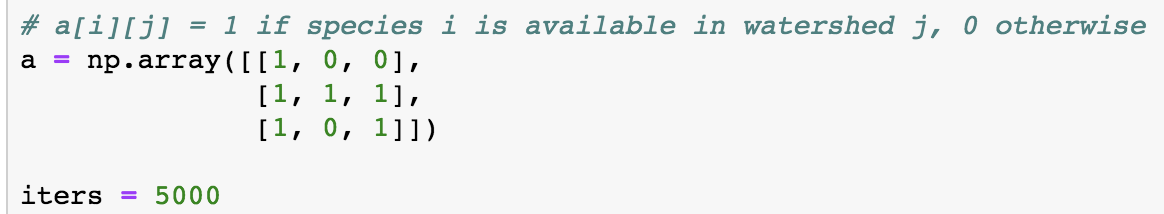
\includegraphics[width=14cm]{pic3.png}

\begin{center}
\begin{tabular}{ |c|c|p{50mm}| } 
 \hline
  & number of iterations to converge & performance  \\ 
 \hline
 optimal solution by scipy & 19 &  \\ 
 \hline
 \rho=0.1 & did not converge in 20000 iterations &  \\ 
 \hline
 \rho=1 & did not converge in 20000 iterations &  \\ 
 \hline
 \rho=10 & 3130 & x=[12995, 165, 531] \newline specie target=[1.45, 3.5, 3.0] \\ 
 \hline
 \rho=100 & 316 & x=[13937, 162, 500]\newline specie target=[1.495, 3.5, 3.0] \\ 
 \hline
 \rho=1000 & 60 & x=[14000, 165, 495]\newline specie target=[1.4976, 3.5, 3.0] \\ 
 \hline
 \rho=10000 & 31 & x=[14000, 165, 495]\newline specie target=[1.4976, 3.5, 3.0] \\ 
 \hline 
 \rho=100000 & 169 & x=[14065, 165, 494]\newlne specie target=[1.5, 3.5, 3.0] \\ 
 \hline 
 \rho=1000000 & 1650 & x=[14065, 165, 494]\newline specie target=[1.5, 3.5, 3.0]\\
 \hline
\end{tabular}
\end{center}
More detailed performance data on\\ https://sites.google.com/mtholyoke.edu/admm-18/jessicas-weekly-report/week-10-nov-20th


\subsubsection{A specific example num\_species = 50, num\_watersheds\_total = 50}
In one example scipy.minimize solve the problem in 643.100438117981 seconds, 413 iterations, with message ``Optimization terminated successfully". \newline

(To replicate this problem, use the 11.28 python code with:

Make up roi curves: np.random.seed(2032)

Make up matrix A and vector b: np.random.seed(6873480)

and no other changes)

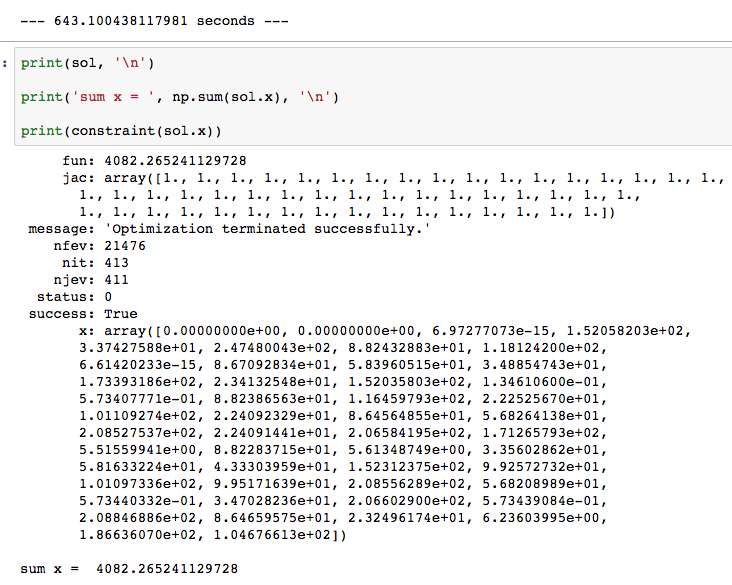
\includegraphics[width=14cm]{pic5.png}

We also tried to use ADMM to solve this problem. This is how long it takes in the first few iterations.

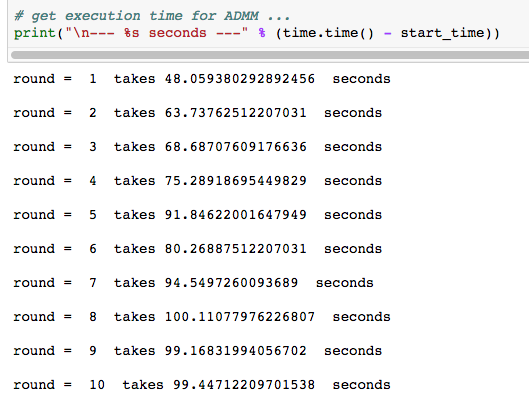
\includegraphics[width=10cm]{pic6.png}

The 11.28 Python code took ADMM 71.5 hours, 1516 iterations to solve this problem, with slightly worse solution than that obtained by scipy.minimize. See 11.28 (2) Python code for details. 

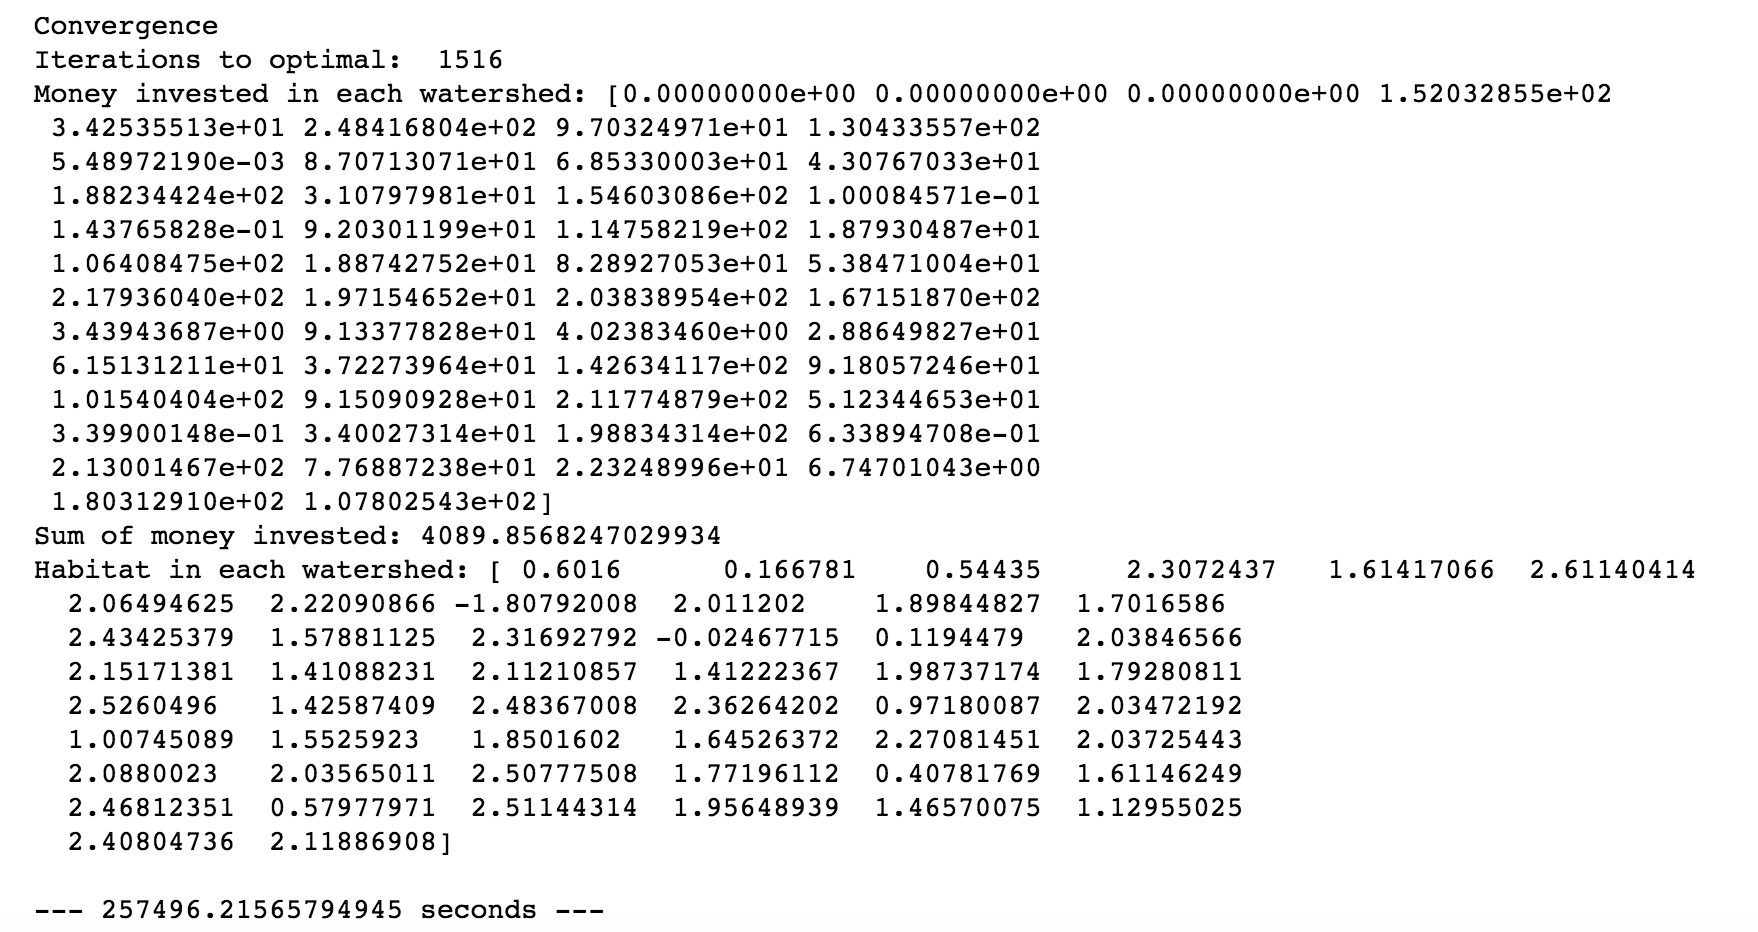
\includegraphics[width=14cm]{pic9.png}

\subsubsection{Observations and thoughts on experiments}

A random observation: In some small-sized problems (num\_species = 5, num\_watersheds\_total = 5), there's an instance where ADMM converges within 32 iterations, scipy.minimize around 55 iterations. Of course scipy.minimize did it much much faster. (we did not time this though). \newline

In all instances we've looked at, ADMM's solution is almost always extremely close to that obtained by scipy.minimize. In some cases, the solution by ADMM is smaller, so better, though not strictly feasible, but maybe the violations were insignificant. Perhaps we can be confident that ADMM give optimal solutions when there is indeed a feasible region, but we are not able to prove optimality by KKT conditions yet. \newline 

As we already know, ADMM is very sensitive to $\rho$. \newline

In \cite{Penalty Parameter}, section 4. Locally Adaptive ADMM for Deterministic Optimization, it seems that the only part that we can try on our problem is Algorithm 2. LA-ADMM. I've tried this on small-sized problems (num\_species = 5, num\_watersheds\_total = 5) by initially setting p = p0 (0.01, 0.1, etc), then set p = 2*p after each iteration. ADMM converges after a small number of iterations, but KKT conditions are not satisfied, and the solution is way worse than that obtained by scipy.minimize. Perhaps ADMM's solution is not optimal when we set $\rho$ this way. The other section of this paper is for stochastic optimization, which I did not look at since our problem is deterministic. \newline

Several papers explaining how to set $\rho$ all depend on the details of the standard form problems. Our problem is not in standard form, so it's tricky to convert those suggestions to what we should do on our problem.  

Perhaps, comparing performance of ADMM and scipy by plotting their number of iterations is not an ideal choice. In the dual update step updating $x$, for complicated enough problems, maybe ADMM will iterate over a lot of times before finding the optimal $x$ (at that step), leading to a large number of iterations till convergence. Maybe this is a problem of applying ADMM on our problem that we should keep in mind.

\section{More experiments}


\textbf{Example 1. ADMM found optimal solution, but KKT conditions are not satisfied.}

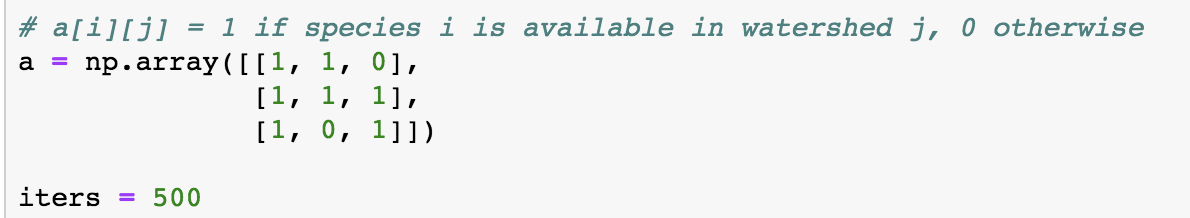
\includegraphics[width=14cm]{pic1.png}

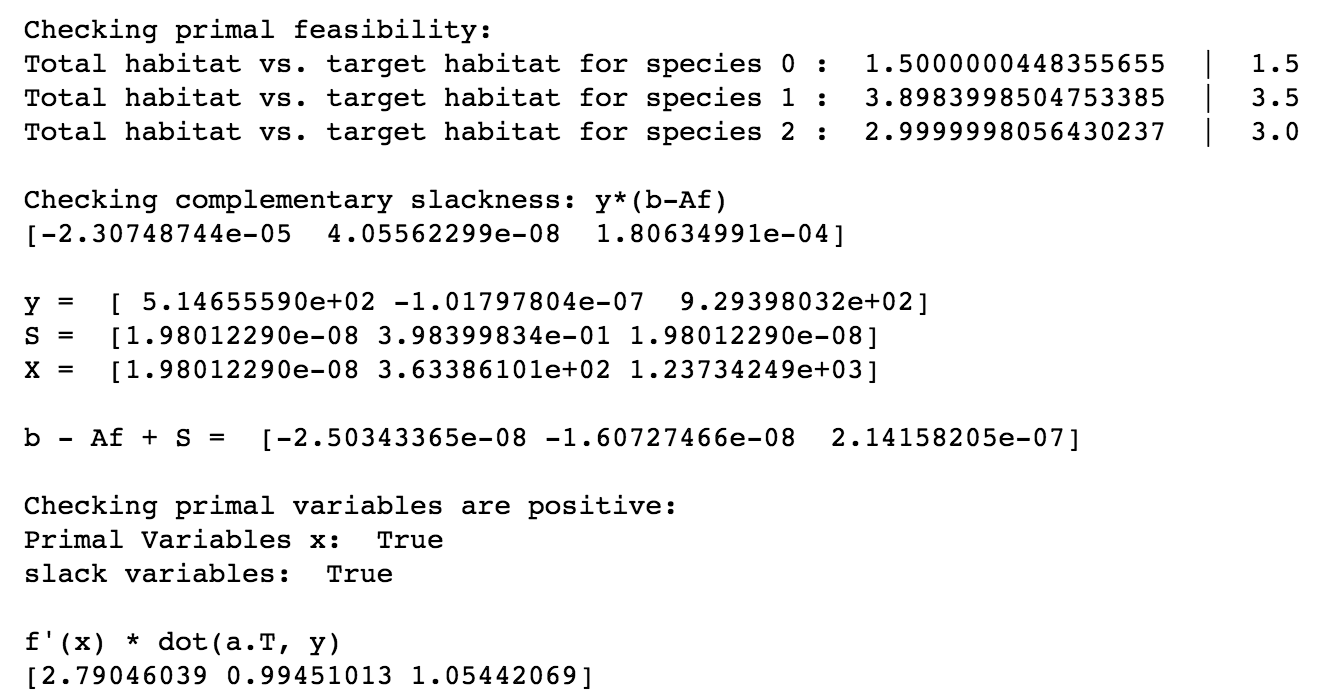
\includegraphics[width=14cm]{pic2.png}

(Iterations to convergence: 370)

\underline{Comment}: 
\begin{itemize}
\item In this case $x_2, x_3 > 0$, by complementary slackness, $w_2=w_3=0$. We want to have: $f'_2(x_2) \sum\limits_{i=1}^3 y_i \cdot a_{i2} \approx 1$, and $f'_3(x_3) \sum\limits_{i=1}^3 y_i \cdot a_{i3} \approx 1$, and we actually have them. \\
\item Besides, $x_1 \approx 0$, so $w_1 x_1 = 0$ for any value of $w_1 \le 0$. There are no other constraints on $w_1$. We can set $w_1$ so that $1 - f'_1(x_1) \sum\limits_{i=1}^3 y_i \cdot a_{i1} + w_1 \approx 0$. 
\\However, we restrict $w_1 \le 0$, so we can't make this expression $\approx 0$. 
\item \color{black} We have $s_2 \neq 0$. By complementary slackness, $z_2 = 0$. We therefore want $y_2 \approx 0$ to satisfy the 2nd complementary slackness, and it's true that $y_2 \approx 0$.
\item We have $s_1,s_3 \approx 0$, so $z_1s_1, z_3 s_3 = 0$, for any values $z_1,z_3 \le 0$. There are no other constraints on $z_1,z_3$. We can set $z_1,z_3$ so that $y_1 + z_1 = y_3 + z_3 = 0$ to satisfy the 2nd complementary slackness condition.
\end{itemize}

\textbf{Example 2. ADMM found optimal solution, but KKT conditions are not satisfied}

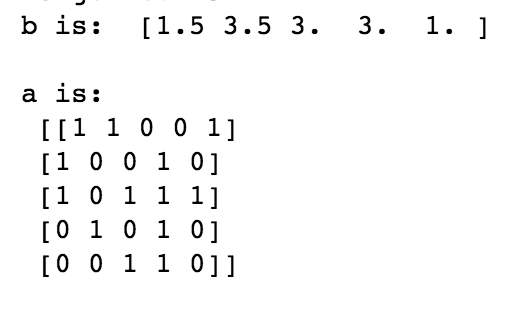
\includegraphics[width=5cm]{pic7.png}

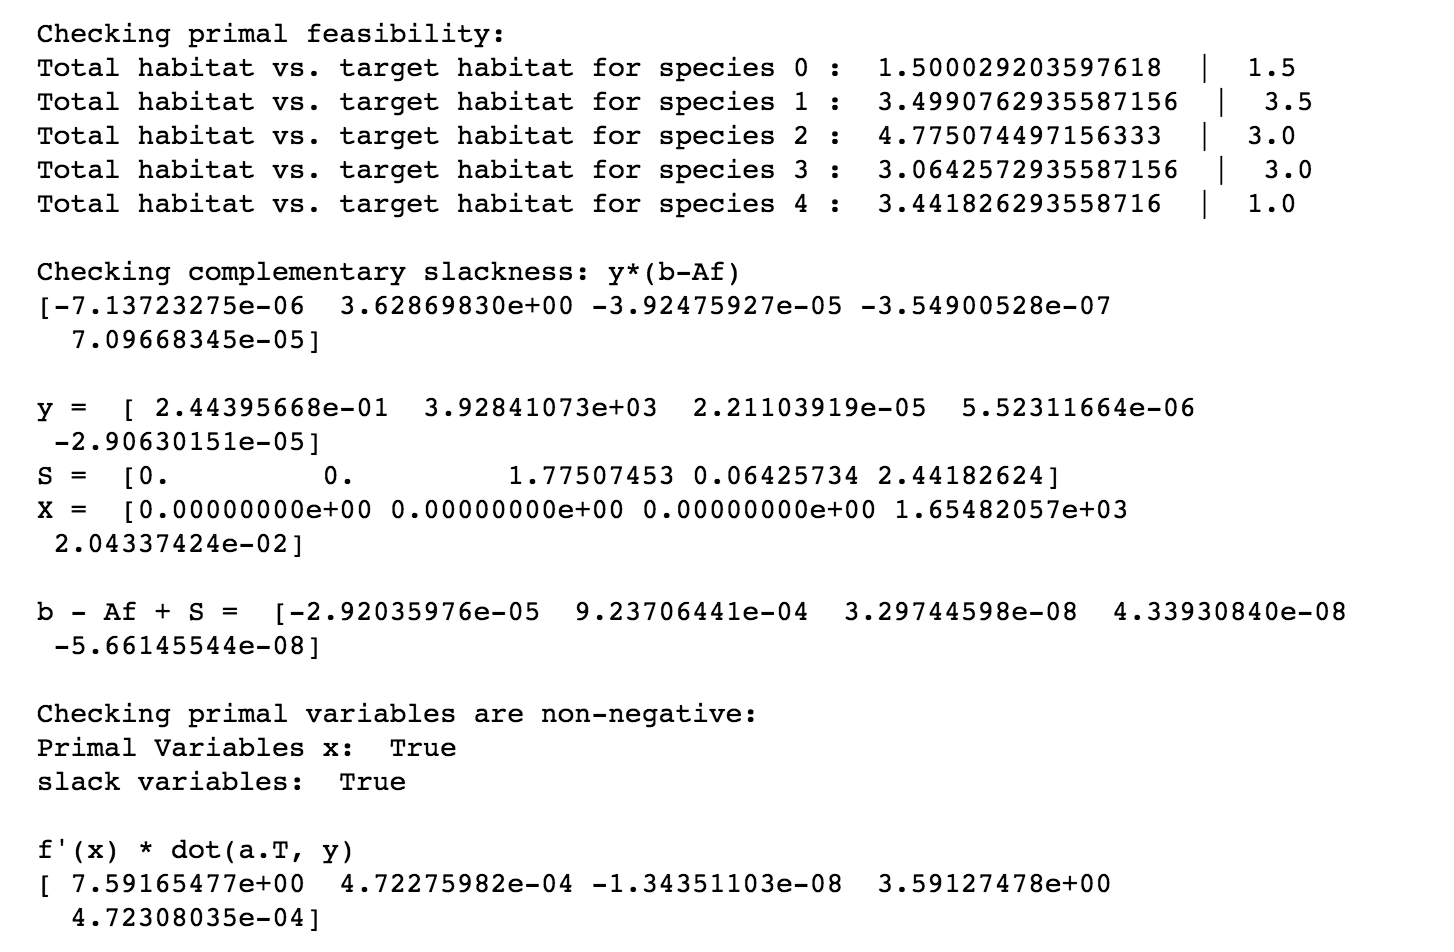
\includegraphics[width=14cm]{pic8.png}

(Iterations to convergence: 107. This solution should be optimal since it is almost exactly the same as the solution obtained by scipy.minimize)\newline

\underline{Comment:}
\begin{itemize}
    \item $x_1,x_2,x_3,x_5 \approx 0$, and we need: $1 \ge f'_k(x_k) \sum\limits_{i=1}^5 y_i \cdot a_{ik}$, for $k = 1, 2, 3, 5$. However we do not.
    \item $x_4 > 0$, so we need $1 = f'_4(x_4) \sum\limits_{i=1}^5 y_i \cdot a_{i4}$, but we do not. 
    \item $s_3, s_4, s_5 > 0$, so we need $y_3,y_4,y_5 \approx 0$, and it's true that $y_3,y_4,y_5 \approx 0$.  
    \item $s_1,s_2 = 0$, so $y_1,y_2$ can have any values.
\end{itemize}

\textbf{Example 3}. ADMM did not find a \underline{feasible} solution.

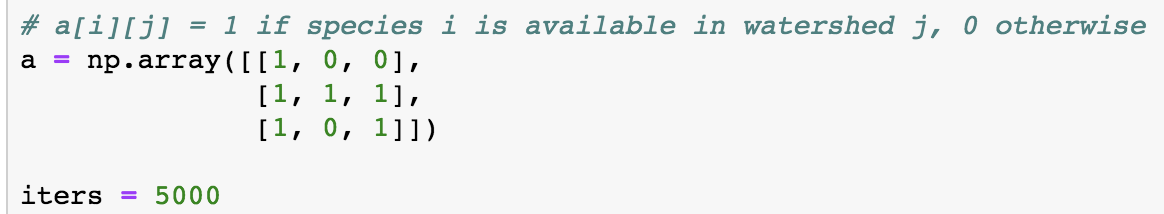
\includegraphics[width=14cm]{pic3.png}

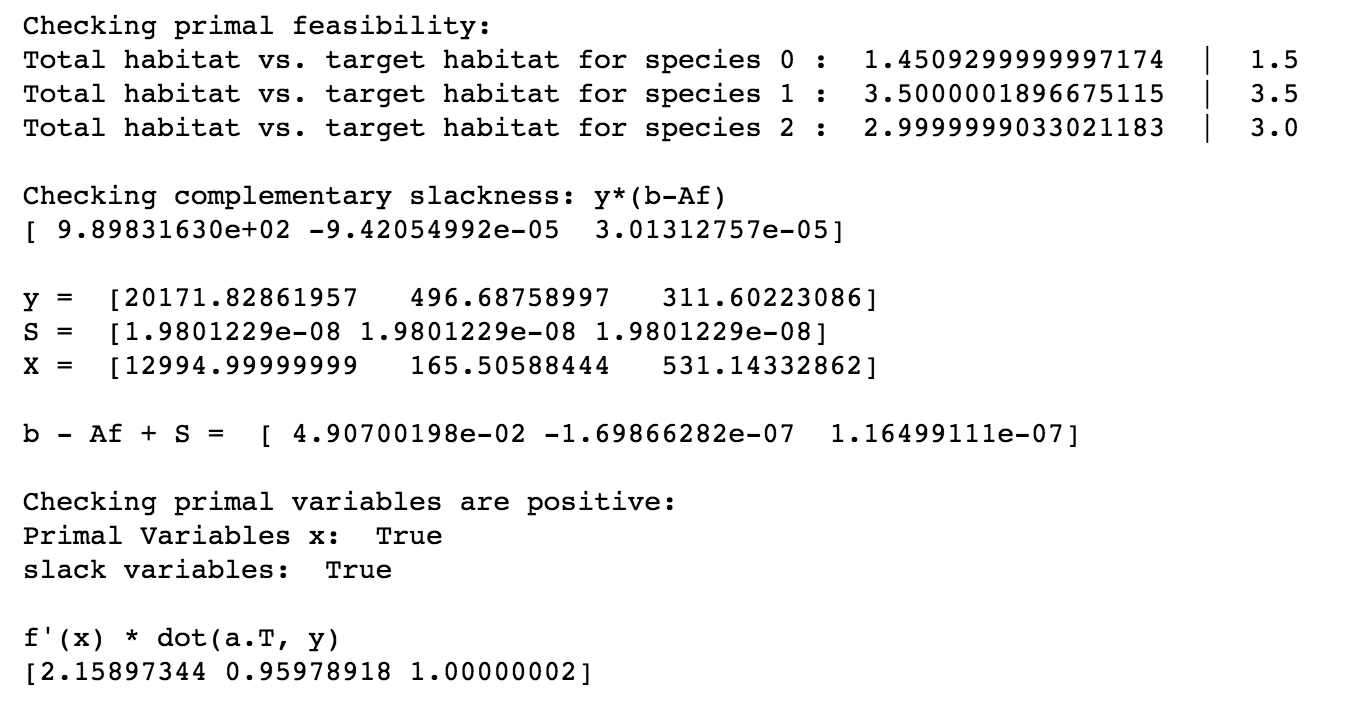
\includegraphics[width=14cm]{pic4.png}

(Convergence, iterations to optimal: 3130)

\underline{Comment}: 
\begin{itemize}
    \item 1st primal feasibility does NOT hold.
    \item Checking complementary slackness $y*(b-Af)$ first component does NOT hold.
    \item We have $s_1,s_2,s_3 \approx 0$, so $z_1s_1 = z_2s_2 = z_3s_3 = 0$ for any values $z_1,z_2,z_3 \le 0$. We can set $z_1,z_2,z_3$ so that $y_1+z_1=y_2+z_2=y_3+z_3=0$ to satisfy the 2nd complementary slackness (can we?)
    \item $x_1 \neq 0$, thus $w_1 = 0$ by complement slackness.\\ We want to have $f'_1(x_1) \sum\limits_{i=1}^m y_i \cdot a_{i1} = 1$, but we do NOT have it.
    \item ($x_1$ is suspiciously too big compared to $x_2$ and $x_3$.)
\end{itemize}

\section{Conclusion \& Future Work}
In this project, we learned about convex optimization and the Alternating Direction Method of Multipliers. In the experiments we have done, ADMM often took much longer time to solve for the optimal solutions compared to scipy optimize, but the solutions obtained by ADMM are usually extremely closed to those by scipy. We suspect that there a few reasons for this problem. First, we did not optimize the code, which may potentially reduce time complexity. Second, the subproblem for finding optimal $x$ in each iteration of the ADMM can be very complicated, which might require many iterations until convergence.\newline
	
In futre work, we would like to optimize and profile the code to see where it is spending the most time at. We will do more experiments on large-scale problems to compare runtime of ADMM versus scipy. One possible comparison is to graph the number of iterations to convergence of both methods as we increase the problem size.\\

We are also interested in understanding the proof of convergence for standard ADMM, and perhaps try to extend it to non-linear constraints problems. As we know, ADMM is very sensitive to $\rho$, but we did not have a systematic way to set $\rho$ for our problem, which may have significantly increased the run time. One possible future direction is to explore these questions, extend the method to non-linear problems, and apply it to more practical applications.\newline

We thank Professor Dan Sheldon for his guidance on this project. This work would have been impossible without his guidance and encouragement. 

\bibliographystyle{abstract}
%\bibliographystyle{alpha}
%\bibliographystyle{plain}
%\begin{small}
%\bibliography{dyck2syt}
%\end{small}

\begin{thebibliography}{99}
\bibitem{ADMM} Boyd, S., Parikh, N., Chu, E., Peleato, B., \& Eckstein, J. (2011). Distributed optimization and statistical learning via the alternating direction method of multipliers. Foundations and Trends® in Machine learning, 3(1), 1-122.

\bibitem{CvxOpt} Boyd, Stephen, and Lieven Vandenberghe. Convex Optimization. Cambridge University Press, 2015.
\bibitem{KKT} http://apmonitor.com/me575/index.php/Main/KuhnTucker
\bibitem{Non linear inequality} http://adl.stanford.edu/aa222/Lecture\_Notes\_files/chapter5\_constrainopt.pdf
\bibitem{Penalty Parameter} Xu, Yi, Mingrui Liu, Qihang Lin, and Tianbao Yang. "ADMM without a Fixed Penalty Parameter: Faster Convergence with New Adaptive Penalization." In Advances in Neural Information Processing Systems, pp. 1267-1277. 2017.

https://papers.nips.cc/paper/6726-admm-without-a-fixed-penalty-parameter-faster-convergence-with-new-adaptive-penalization.pdf

\end{thebibliography}

\end{document}

